%! TeX root = master.tex
% !TEX program = lualatex

\lecture{3}{2026-09-24}{Access control basics and DAC}{}
\chapter{Access Control}
\label{ch:access-control}

\section{Introduction to access control}

\subsection{What is access control?}

In the physical world, access control is everywhere: a key in a lock, a badge on a reader, a turnstile in a metro station.

The digital world has exactly the same needs, and we will see that the mechanisms are conceptually similar.

\begin{definition}[Access control]
A security mechanism that ensures that \textbf{all accesses and actions on objects by principals are within the security policy}.
\end{definition}

An access control system must be able to answer questions such as:
\begin{itemize}
    \item Can Alice read the file \texttt{/users/Bob/readme.txt}?
    \item Can Bob open a TCP socket to \texttt{http://www.abc.com/}?
    \item Can Charlie write to row 15 of the table \texttt{GRADES}?
\end{itemize}

The answer to each question is binary: either the access is \textbf{authorized} (the principal \emph{has permission}), or it is \textbf{unauthorized} (\emph{access denied}). The goal is that \textbf{only events within the security policy} actually happen.

\begin{remark}
Recall the vocabulary of Chapter 1\ref{ch:intro-security}: the \emph{principals} (subjects) are the entities acting on the system, the \emph{assets} (objects) are the things to protect, and the \emph{security policy} says which principal may do what on which asset. Access control is the mechanism that \emph{enforces} this policy.
\end{remark}

\subsection{Why is access control so important?}

Access control is the \textbf{first line of defence}. As a consequence, it is used at \emph{every} layer of a system:

\begin{table}[h]
\centering
\begin{tabular}{@{}p{3.2cm}p{9.5cm}@{}}
\toprule
\textbf{Layer} & \textbf{Examples of what access control protects} \\
\midrule
Applications & Online social networks, e-mail servers, cloud storage \\
Middleware & Database management systems (DBMS) \\
Operating system & Files, directories, ports, \dots \\
Hardware & Memory, registers, privilege levels \\
\bottomrule
\end{tabular}
\caption{Access control is used at every layer of the system stack.}
\end{table}

\subsection{Where does access control fit? Authentication vs.\ authorization}

Access control is usually split into two steps:

\begin{enumerate}
    \item \textbf{Authentication}: the system must \emph{bind the actor to a principal}. A principal is an abstract entity that is authorized to act (a user, a connection, a process, \dots).  
    \item \textbf{Authorization}: the system must \emph{decide whether the principal is authorized} to perform the requested action on the requested object.
\end{enumerate}

\begin{remark}
The mechanisms that perform authentication \textbf{and} authorization are part of the \textbf{Trusted Computing Base} (TCB): if they fail, the security policy may be violated.
\end{remark}

\subsection{Implementing access control: the reference monitor}

\paragraph{What NOT to do: ``checks soup''.} A naive implementation sprinkles checks all over the program, each one implementing the policy \emph{in-line}:

\begin{verbatim}
# some code that needs to access file3.txt
if (action == read) and ((userID == Alice) or (userID == Bob)):
    open(file3.txt, 'r')
elif (action == write) or (userID == Bob):
    open(file3.txt, 'w')
else:
    print("The user does not have access to file3.txt")
\end{verbatim}

This is a bad design: the policy is scattered everywhere, which makes it hard to audit, hard to change, and very error-prone. (The example above even contains a bug: the \texttt{write} branch uses an \texttt{or}, so \emph{anybody} can write the file!) It is the opposite of \emph{economy of mechanism}.

\paragraph{What you SHOULD do: systematic calls to a reference monitor.} Throughout the program, add checks that \textbf{call a central monitor}. The checks state which authorization is required and provide \emph{evidence} about the principal and the object; the central subsystem (the \textbf{reference monitor}) decides whether the check passes.

\begin{verbatim}
if ( subject.isPermitted("user:delete:jsmith") ) {
    // delete the 'jsmith' user
} else {
    // don't delete 'jsmith'
}
\end{verbatim}
The application does not contain the policy: it only asks the monitor.

\begin{remark}
The reference monitor is how \textbf{complete mediation} is put in practice (every access goes through the monitor), and keeping it small and central follows \textbf{economy of mechanism}. The slides ask, with a question mark, whether this violates \textbf{least common mechanism}: a central monitor \emph{is} a mechanism shared by all users. This is a typical example of \emph{tension between principles}, which must be weighed explicitly rather than ticked off blindly.
\end{remark}

\subsection{Who decides the access policy? DAC vs.\ MAC}

There are two fundamentally different answers to the question ``who defines who can access what?''.

\begin{table}[h]
\centering
\begin{tabular}{@{}p{3cm}p{5.2cm}p{5.2cm}@{}}
\toprule
 & \textbf{Discretionary (DAC)} & \textbf{Mandatory (MAC)} \\
\midrule
\textbf{Who sets permissions} & The \textbf{owner} of each object assigns permissions & A \textbf{central security policy} assigns permissions \\[4pt]
\textbf{Key idea} & Ownership of resources & Organizations with a need for central control \\[4pt]
\textbf{Typical uses} & Windows, Linux, macOS; social networks; cloud file sharing &
Military (focus on confidentiality); hospitals (confidentiality \emph{and} integrity); banking (focus on integrity) \\
\bottomrule
\end{tabular}
\caption{Discretionary vs.\ mandatory access control.}
\end{table}

\section{Discretionary Access Control (DAC)}

\begin{definition}[Discretionary Access Control]
An access control approach in which the \textbf{owners of the objects establish the permissions} on them.
\end{definition}

\subsection{Historical motivation: Lampson's protection}

DAC policies were conceptualized by B.\ Lampson in \emph{Protection} (Proc.\ 5th Princeton Conf.\ on Information Sciences and Systems, 1971; reprinted in ACM Operating Systems Review 8(1), 1974).

The original motivation for protection mechanisms in computers was to keep \emph{one user's malice or error} from harming another user. Harm can be inflicted by:
\begin{enumerate}
    \item[a)] destroying or modifying another user's data;
    \item[b)] reading or copying another user's data without permission;
    \item[c)] degrading the service another user gets (e.g., using up all the disk space or getting more than a fair share of the processing time; an extreme case is crashing the system).
\end{enumerate}
Lampson adds that all these reasons are just as strong if the word ``user'' is replaced by ``\emph{program}'': a program (e.g., downloaded malware) can be as dangerous as a malicious user.

These three kinds of harm map directly onto the CIA triad: (b) is a confidentiality violation, (a) an integrity violation, (c) an availability violation.

\subsection{The Access Control Matrix}

In a real system there are many subjects, many objects, and many combinations of permissions between them. How can we reason about them? DAC policies are conceptualized as an \textbf{access control matrix}.

\begin{definition}[Access control matrix]
An \textbf{abstract representation of all permitted triplets} (subject, object, access right) within a system. Rows are subjects, columns are objects, and each cell contains the set of operations the subject is allowed to perform on the object.
\end{definition}

\begin{itemize}
    \item \textbf{Subjects} (principals): entities within an IT system: a user, a process, a service.
    \item \textbf{Objects} (assets): resources that (some) subject may access or use: a file, a folder, a row in a database, the system's memory, a machine on the network, a printer, a page of a website.
    \item \textbf{Operations}: in the abstract, subjects can \emph{observe} and/or \emph{alter} objects: \texttt{read}, \texttt{write}, \texttt{append}, \texttt{execute}.
\end{itemize}

\begin{example}
Let $S = \{\text{Alice}, \text{Bob}\}$, $O = \{\text{file1}, \text{file2}, \text{file3}\}$ and $A = \{\text{read}, \text{write}\}$.

\begin{table}[h]
\centering
\begin{tabular}{@{}lccc@{}}
\toprule
 & \textbf{file1} & \textbf{file2} & \textbf{file3} \\
\midrule
\textbf{Alice} & read, write &  & read \\
\textbf{Bob} &  & read, write & read, write \\
\bottomrule
\end{tabular}
\caption{An access control matrix.}
\end{table}

Can Alice read file1? \emph{Yes.} Can Bob write file1? \emph{No} (empty cell: no permission). Can file3 be written by Alice? \emph{No} (she only has \texttt{read}).
\end{example}

\begin{remark}[Fail-safe defaults]
An empty cell means \emph{no permission}. This is the whitelist approach of fail-safe defaults: everything that is not explicitly granted is denied.
\end{remark}

\subsubsection{Why the matrix is not implemented directly}

The access control matrix is an \textbf{abstract concept}, not meant for direct implementation. With $f$ files and $u$ users it takes $O(f \cdot u)$ space. For a system with $629\,601$ files:

\begin{table}[h]
\centering
\begin{tabular}{@{}lr@{}}
\toprule
\textbf{Setting} & \textbf{Matrix size} \\
\midrule
1 bit per file, 1 user & $\approx 78$\,KB \\
3 bits per file (r/w/x), 1 user & $\approx 236$\,KB \\
3 bits per file, 10 users & $\approx 2.36$\,MB \\
\bottomrule
\end{tabular}
\end{table}

Beyond raw size, there are more issues:
\begin{itemize}
    \item The matrix is usually \textbf{very sparse}, hence wasteful.
    \item It is \textbf{inefficient to access}: it would have to be kept in fast memory.
    \item \textbf{Extensibility}: what happens when a file or a user is added?
\end{itemize}

The matrix can be stored in two natural ways: by \emph{column} (permissions attached to objects: \textbf{ACLs}) or by \emph{row} (permissions attached to subjects: \textbf{capabilities}). Role- and group-based access control are ways of \emph{factoring} the subjects.

\subsection{Access Control Lists (ACLs)}

\begin{definition}[Access Control List]
An implementation of the access control matrix that \textbf{associates permissions to objects}: each object stores the list of (subject, rights) pairs that are allowed to access it. \textbf{Blank cells are not stored.}
\end{definition}

For the matrix above:
\begin{align*}
\text{file1} &: \{(\text{Alice}, \text{read/write})\}\\
\text{file2} &: \{(\text{Bob}, \text{read/write})\}\\
\text{file3} &: \{(\text{Alice}, \text{read}), (\text{Bob}, \text{read/write})\}
\end{align*}

\begin{table}[h]
\centering
\begin{tabular}{@{}p{6.3cm}p{6.7cm}@{}}
\toprule
\textbf{Advantages} & \textbf{Drawbacks} \\
\midrule
Can be stored close to / with the resource & Difficult to check at runtime \\
Easy to determine \emph{who can access a resource} & Difficult to audit \emph{all the rights of a user} \\
Easy to \emph{revoke rights by resource} & Difficult to remove all permissions from a user (better remove their authentication!) \\
 & Difficult delegation \\
\bottomrule
\end{tabular}
\caption{Pros and cons of ACLs.}
\end{table}

\subsection{Role Based Access Control (RBAC)}

Systems have \textbf{too many subjects}, and they come and go. This leads to large, dynamic ACLs that are painful to maintain. However, subjects are often \emph{similar to each other}: e.g., a doctor has the same privileges as another doctor. RBAC exploits this:

\begin{definition}[Role Based Access Control]
\begin{enumerate}
    \item \textbf{Assign permissions to roles};
    \item \textbf{assign roles to subjects};
    \item subjects \textbf{select an active role}: they hold the permissions of the active role.
\end{enumerate}
\end{definition}

Roles add a level of indirection: when an employee changes job, we change their role assignment rather than editing the ACL of every object.

\vspace{-5pt}
\paragraph{Problems of RBAC.}
\begin{enumerate}
    \item \textbf{Role explosion}: the temptation to create very fine-grained roles removes the benefit of RBAC (we end up with roughly as many roles as subjects).
    \item \textbf{Limited expressiveness} of simple RBAC: it is hard to implement least privilege precisely, and some roles are \emph{relative}: ``Alice's doctor'' versus ``any doctor''.
    \item \textbf{Separation of duty is difficult}: e.g., ``two doctors are needed to authorize a procedure''. The RBAC mechanism itself needs to ensure that the two doctors are \emph{distinct}, which a plain role-to-permission mapping cannot express.
\end{enumerate}

\subsection{Group Based Access Control}

Another way to factor subjects: some permissions are \textbf{always needed together} (e.g., access to sockets and to the network interface go hand in hand).

\begin{definition}[Group Based Access Control]
\begin{enumerate}
    \item \textbf{Assign permissions} to access objects \textbf{to groups};
    \item \textbf{assign subjects to groups};
    \item subjects hold \textbf{the permissions of all their groups}.
\end{enumerate}
\end{definition}

\begin{remark}[Groups vs.\ roles]
The difference with RBAC is subtle but important: in group-based access control a subject has the \emph{union} of the permissions of \emph{all} its groups at all times, whereas in RBAC the subject activates \emph{one role at a time} and holds only its permissions, which helps enforce least privilege.
\end{remark}

\paragraph{Negative permissions.} To express fine-grained policies, group-based systems often add \textbf{negative permissions} (explicit denials), e.g., ``everyone in group1 may read, except Alice''.

\begin{center}
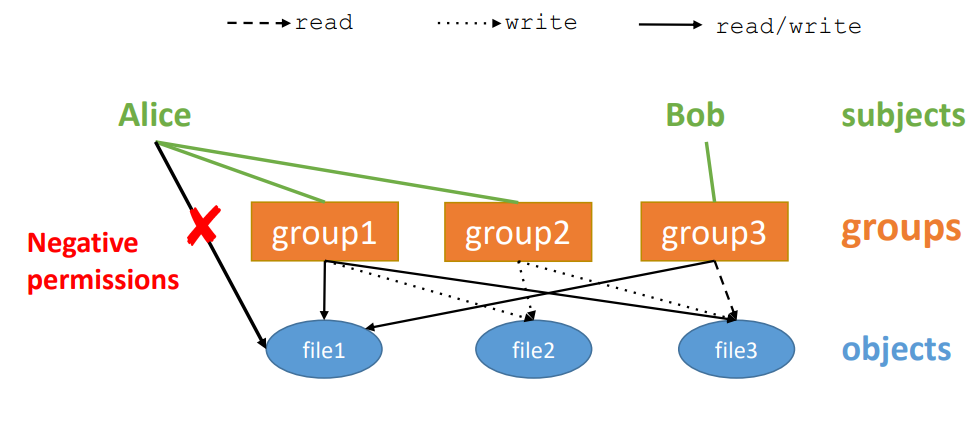
\includegraphics[width=0.6\linewidth]{images/img_20261002_171837.png}
\end{center}

\begin{remark}[What do we check first?]
\textbf{Negative permissions must be checked first.} Otherwise a positive permission obtained through another group could grant the access before the denial is ever seen. Evaluating denials first is also consistent with \textbf{fail-safe defaults}. (Windows does exactly this; see below.)
\end{remark}

\subsection{Capabilities}

\begin{definition}[Capability]
An implementation of the access control matrix that \textbf{associates permissions to subjects}: each subject holds the list of (object, rights) pairs it is allowed to use. A capability is an \emph{unforgeable} reference to an object that carries the right to use it; holding it is what gives the authority.
\end{definition}

For the same matrix:
\begin{align*}
\text{Alice} &: \{(\text{file1}, \text{read/write}), (\text{file3}, \text{read})\}\\
\text{Bob} &: \{(\text{file2}, \text{read/write}), (\text{file3}, \text{read/write})\}
\end{align*}
Again, blanks are not stored.

\vspace{40pt}

\begin{table}[h]
\centering
\begin{tabular}{@{}p{6.3cm}p{6.7cm}@{}}
\toprule
\textbf{Advantages} & \textbf{Drawbacks} \\
\midrule
Can be stored \emph{with the subject} (portable!) & \emph{Revoking} the permission on one object is hard \\
Easy to audit \emph{all the permissions of a subject} & \emph{Transferability}: once a capability is given, how can we prevent sharing? \\
Delegating is ``simple'' (hand over the capability) & \emph{Authenticity}: how can we check that a capability is genuine (not forged)? \\
\bottomrule
\end{tabular}
\caption{Pros and cons of capabilities.}
\end{table}

\begin{remark}[ACLs vs.\ capabilities: mirror images]
The pros and cons are exactly mirrored. ACLs make \emph{per-object} questions easy (who can access this file? revoke access to it) and \emph{per-subject} questions hard. Capabilities make \emph{per-subject} questions easy (what can Alice do? delegate) and \emph{per-object} questions hard. This mirrors the two ways of storing a sparse matrix: by column or by row.
\end{remark}

\section{Ambient authority and the confused deputy}

\subsection{Ambient authority}

\begin{definition}[Ambient authority]
A subject uses \textbf{ambient authority} if, for an action to succeed, it \textbf{only needs to specify the operation and the names of the involved objects}. The subject holding the authority is \emph{implicit}.
\end{definition}

\begin{example}
\texttt{open("file1", "rw")}: the subject is missing from the call; it is implicitly the \emph{owner of the process}.
\end{example}

\begin{itemize}
    \item \textbf{Advantage}: usability. There is no need to repeat the subject all the time.
    \item \textbf{Drawbacks}: \textbf{least privilege becomes harder to enforce} (the process uses \emph{all} the authority of its owner for \emph{every} action), and the program itself \textbf{cannot check permissions} on behalf of the party that actually requested the action. This leads to the confused deputy problem.
\end{itemize}

\subsection{The confused deputy problem}

\begin{definition}[Confused deputy problem]
A problem of ambient authority: a \textbf{privileged program can be tricked into misusing its authority} on behalf of a less privileged requester.
\end{definition}

\begin{example}[The pay-per-use compiler]
(The classic example, due to N.\ Hardy.) A compiler is offered as a pay-per-use service. It receives two file names \texttt{(input, output)}. It compiles the program \texttt{input}, then:
\begin{itemize}
    \item writes the \textbf{usage} (what the user owes) into the file \texttt{bill};
    \item writes the \textbf{errors} into the file \texttt{output}.
\end{itemize}

The compiler's own access rights are those of the service. The ACLs are:
\begin{align*}
\texttt{input} &: \{(\text{Alice}, \text{write}), (\text{Compiler}, \text{read})\}\\
\texttt{output} &: \{(\text{Alice}, \text{read}), (\text{Compiler}, \text{read/write})\}\\
\texttt{bill} &: \{(\text{Alice}, \text{read}), (\text{Compiler}, \text{read/write})\}
\end{align*}

\textbf{Can Alice change the bill and avoid paying?} Not directly: Alice only has \texttt{read} on \texttt{bill}. But Alice calls the compiler with arguments \texttt{(input, bill)}, i.e., she chooses \texttt{bill} as the \emph{output} file. The compiler compiles \texttt{input} and writes the errors into ``\texttt{output}'' $=$ \texttt{bill}. The compiler is allowed to write \texttt{bill}, so the write succeeds and \textbf{the bill is corrupted}.
\end{example}

Why does this happen? The compiler \emph{never checks} whether Alice herself would be allowed to write the file she designated as output: it uses its own (ambient) authority to do so. The \emph{designation} of the object (the name chosen by Alice) is separated from the \emph{authority} used to act on it.

\paragraph{How to avoid confused deputies.} This is a real problem, because ambient authority is used for convenience in many real systems: OS services, web servers, \dots Solutions:
\begin{enumerate}
    \item \textbf{Re-implement access control in the privileged process} (e.g. before writing in \textit{output}, the compiler check if output = bill);
    \item \textbf{let the privileged process check the authorization of Alice} (not only its own);
    \item \textbf{use capabilities}.
\end{enumerate}

\begin{example}[The compiler with capabilities]
The compiler holds a capability to the file \texttt{bill} (for its own use). To compile, Alice must \emph{give} the compiler a capability to the debugging file \texttt{output}. Alice only holds a read capability on \texttt{bill}, so she \textbf{cannot hand over a capability for writing on \texttt{bill}}. Since the authority travels together with the name of the object, nobody can be confused.
\end{example}

\begin{remark}[Exam hints on the confused deputy]
Do not just throw the keyword ``confused deputy'' (or ``ambient authority'') at a question: link it to the problem at hand. Identify (1) the privileged \emph{deputy}, (2) the less privileged \emph{requester} who controls what the deputy is asked to do, and (3) the action that the requester could not perform alone but that the deputy performs with its own authority. In a past MCQ about a room booking system, the maintenance team (the deputy) cancelling all bookings on a \emph{wrong report} was debated precisely because the question must be read in terms of these three elements.
\end{remark}

\section{Summary of the DAC concepts}

\begin{itemize}
    \item \textbf{Discretionary Access Control}: owners establish permissions.
    \item Conceptualized as an \textbf{access control matrix} (abstract; not implemented directly).
    \item Implemented in two flavours: \textbf{access control lists} (permissions associated to objects) and \textbf{capabilities} (permissions associated to subjects).
    \item Roles and groups factor many subjects into a few classes of subjects.
    \item When relying on access control, always think about \textbf{confused deputies}.
\end{itemize}

\section{DAC in practice: Linux (UNIX) and Windows}

Many of the systems we use every day rely on DAC: social networks, cloud file-sharing systems, and operating systems.

\subsection{UNIX: principals and groups}

\begin{itemize}
    \item \textbf{User identities} (UIDs) and \textbf{group identities} (GIDs): originally 16-bit, now 32-bit numbers. Some UIDs are special (e.g., $0$ for root, and the special ``nobody'' user).
    \item \textbf{User information}: each user has their own directory \texttt{/home/username}. User accounts are listed in \texttt{/etc/passwd}, one line per user with the format
    \begin{center}
    \texttt{username:password:UID:GID:info:home:shell}
    \end{center}
    \item Users belong to \textbf{one or more groups}: a \emph{primary} group (given in \texttt{/etc/passwd}) and other groups (listed in \texttt{/etc/group}).
\end{itemize}

\subsubsection{Security architecture}

\begin{itemize}
    \item \textbf{Everything is a file} (regular files, directories, devices, \dots), so one mechanism protects everything.
    \item Each user \textbf{owns} a set of files.
    \item Each file has a simple \textbf{Access Control List} expressing the policy for that file.
    \begin{itemize}
        \item The owner can modify the permissions of the file, but \textbf{cannot give away ownership}.
        \item System files are owned by special users that can perform system operations.
    \end{itemize}
    \item All processes launched by a user run \textbf{with that user's privileges}: this is \textbf{ambient authority}!
\end{itemize}

\subsubsection{File ACLs: the 9 permission bits}

Each file is assigned an \textbf{owner UID} and a \textbf{GID}, and has \textbf{9 permission bits}: 3 actions (\textbf{r}ead, \textbf{w}rite, e\textbf{x}ecute) for 3 classes of subjects (\textbf{owner}, \textbf{group}, \textbf{other}). Besides these there are 3 special attributes: \textbf{suid}, \textbf{sgid} and \textbf{sticky}.

\begin{verbatim}
drwxrwxr-x 1 catronco catronco 4096 Sep 16 14:23 exampledir
-rwxrwxrw- 1 catronco catronco 8600 Sep 15 15:20 hello
-rw-rw-rw- 1 catronco catronco  150 Sep 15 15:14 hello.c
-rw-rw--w- 1 catronco catronco   45 Sep 15 15:07 test1.txt
\end{verbatim}

Reading a line from left to right: the \textbf{type} (\texttt{d} for directory, \texttt{-} for a regular file), the three \textbf{owner} bits, the three \textbf{group} bits, the three \textbf{other} bits, the number of \textbf{links}, the \textbf{owner}, the \textbf{group}, the \textbf{size}, the \textbf{last modification} date and the \textbf{file name}. For example, \texttt{-rw-rw--w-} means: owner may read and write, group may read and write, others may only write.

\paragraph{Different semantics for files and directories.}

\begin{table}[h]
\centering
\begin{tabular}{@{}lp{5.2cm}p{5.2cm}@{}}
\toprule
\textbf{Bit} & \textbf{On a file} & \textbf{On a directory} \\
\midrule
\texttt{r} (read) & Read the content & \textbf{List} the files in the directory \\
\texttt{w} (write) & Modify the content & \textbf{Add} (create) files \\
\texttt{x} (execute) & Run the file as a program & \textbf{Traverse} the directory (\texttt{cd}, and access what is inside by path) \\
\bottomrule
\end{tabular}
\caption{Semantics of the permission bits on files vs.\ directories.}
\end{table}

\begin{remark}[Directory permissions matter on the whole path]
To access \texttt{/a/b/c.txt} one needs the \texttt{x} (traverse) permission on \texttt{/}, \texttt{/a} and \texttt{/a/b}, on top of the right permission on \texttt{c.txt} itself. Creating, deleting or renaming a file is governed by the \texttt{w} (and \texttt{x}) bits of the \emph{containing directory}, not of the file. This is a classic trap in exercises.
\end{remark}

\paragraph{Changing permissions.} The owner can change the permissions of a file with \texttt{chmod}, either symbolically (\texttt{+r}, \texttt{-w}, \dots) or in octal. In octal, read $=4$, write $=2$, execute $=1$ for each of the three triplets, so \texttt{666} $=$ \texttt{rw-rw-rw-} and \texttt{662} $=$ \texttt{rw-rw--w-}. The special bits are written with a fourth leading digit: \texttt{4000} for suid, \texttt{2000} for sgid and \texttt{1000} for sticky. For example, \texttt{+t} or \texttt{1666} sets the sticky bit and \texttt{+s} or \texttt{4666} sets suid.

\subsubsection{How UNIX checks an access}

The kernel compares the \textbf{UID/GID of the process} trying to perform the action with the \textbf{state of the file} (owner, group, mode bits). \textbf{The order matters}:
\begin{enumerate}
    \item If the UID says you are the \textbf{owner}: check the \textbf{owner} bits.
    \item Otherwise, if your \textbf{group} is the file's group: check the \textbf{group} bits.
    \item Otherwise, check the \textbf{other} bits.
\end{enumerate}

\begin{remark}
Only the \emph{first matching class} is used. If you are the owner, the owner bits apply even if the group or other bits are more permissive (so an owner can be \emph{denied} an access that his group is granted). The one exception is the \textbf{root user, who is never denied access}.
\end{remark}

\subsubsection{Super users: root}

\begin{itemize}
    \item Special \textbf{root} user account, with \textbf{user ID 0}.
    \item Accesses system files and performs special operations.
    \item Can access anything: (almost all) security checks are disabled.
    \item \textbf{root is in the TCB!}
\end{itemize}

\textbf{Never log in as root} (some distributions even assign it no password). Use the \texttt{sudo} or \texttt{su} commands instead. This is the least privilege principle at work: operate as an ordinary user and elevate only when needed.

\begin{remark}[\texttt{su} vs.\ \texttt{sudo}]
The slide asks about the difference. Briefly: \texttt{su} (``switch user'') opens a session as another user and requires \emph{that user's} password; \texttt{sudo} runs a \emph{single command} with the privileges of another user (root by default) after the \emph{caller} authenticates with their own password, if the policy (\texttt{/etc/sudoers}) allows it, and it \textbf{logs} each use (compromise recording). In \texttt{sudo su catronco}, \texttt{su} runs as root, which does not need \texttt{catronco}'s password.
\end{remark}

Normal users also need to access \textbf{system services}, but these services must run with system privileges. This is solved with the \textbf{suid/sgid} mechanism.

\subsubsection{Special rights: suid and sgid}

\begin{definition}[Setuid and setgid]
The \textbf{setuid} and \textbf{setgid} bits indicate that an executable file is run not with the privileges of the user who launches it, but with the privileges of the file's owner user (setuid) or owner group (setgid).
\end{definition}

This is especially useful for programs that need root privileges while respecting \textbf{least privilege}: instead of giving the user root, the user is given a single, well-defined program that runs with elevated privileges. The typical example is changing one's password:

\begin{verbatim}
ls -l /bin/passwd
-rwsr-xr-x. 1 root root 27768 Aug 20 2020 /bin/passwd
\end{verbatim}

The \texttt{s} in place of the owner's \texttt{x} indicates the setuid bit. Any user can run \texttt{passwd}, which runs as root and can therefore write the protected password file, but only in the way the program allows.

\begin{remark}[Setuid root programs are dangerous]
How do you know that a suid program does what it is meant to do, \textbf{and only what it is meant to do}? A setuid-root program runs with full root privileges, so any bug in it can be exploited by the user who launches it. \textbf{Setuid root programs are therefore part of the TCB} and must be kept small and audited (economy of mechanism). Imagine what would happen if a general-purpose interpreter such as \texttt{python2.7} were setuid root: anyone could run arbitrary code as root. (See Chen, Wagner, Dean, \emph{Setuid Demystified}, USENIX Security 2002; Kamp and Watson, \emph{Jails: Confining the omnipotent root}, 2000.)
\end{remark}

\begin{remark}[Exam pitfalls on setuid]
Past midterm feedback highlights the following errors:
\begin{itemize}
    \item \textbf{Setuid applies to executables}, i.e., to the \emph{program}, not to a (non-executable) data file.
    \item Use the \textbf{correct notation}: a program owned by \texttt{dave} that members of group \texttt{managers} may run and others may read is \texttt{-rwsr-xr-{}-}.
    \item Do \emph{not} ``fix'' a permission problem by making a sensitive file readable/writable by everybody: this removes any notion of access control on it and violates several security principles.
\end{itemize}
\end{remark}

\begin{example}[Exam-style: emergency deletion program]
Tropyota wants the CEO Carla (group \texttt{managers}) to be able to run an emergency program deleting the secret plans, which only the \texttt{designers} may read or modify. The configuration is
\begin{verbatim}
-rwxr-xr-- dave managers   program_to_delete_plans
-rw-rw---- dave designers  hybris_plans.dwg
\end{verbatim}
\textbf{Does it work?} No: Carla can \emph{execute} the program (group \texttt{managers} has \texttt{r-x}), but with ambient authority the process runs \emph{with Carla's privileges}, and Carla (not in \texttt{designers}) has no access to the plans. \textbf{Fix}: set the \textbf{setuid bit on the program}, giving \texttt{-rwsr-xr-{}-}, so that it runs with the privileges of its owner Dave, who can access the plans.

\textbf{Least privilege?} Still not satisfied: \emph{every} manager (not only the CEO) can run the program, and the program runs with all of Dave's privileges, which is more than strictly necessary.
\end{example}

\subsubsection{Special rights: the sticky bit}

The sticky bit (\texttt{chmod +t}) is also called the \textbf{restricted deletion bit}.
\begin{itemize}
    \item \textbf{On directories}: it prevents unprivileged users from \emph{removing or renaming} a file in the directory unless they own the file. Example: the \texttt{/tmp} folder, which is writable by everyone, but where users can only delete or rename \emph{their own} files.
    \item \textbf{On files}: historically, it kept a program in swap for faster loading. On current Linux, the bit is ignored for files.
\end{itemize}

\begin{remark}
Recall the \texttt{/tmp} symlink attack of the \emph{least common mechanism} example: \texttt{/tmp} is a shared mechanism. The sticky bit limits what users can do to one another's files there, but sharing a writable directory remains risky.
\end{remark}
\enlargethispage{3\baselineskip}
\subsubsection{Special user: nobody}

\texttt{nobody} is a special user (UID $-2$ in the slides) that \textbf{owns no files and belongs to no group of users}. It is a safer user to run code you do not know or trust (particularly obfuscated code), since it \textbf{limits the damage} if the code misbehaves or gets compromised: another application of least privilege.
\newpage
\subsection{Windows}

\begin{itemize}
    \item \textbf{Principals}: users, machines, groups, \dots
    \item \textbf{Objects}: files, Registry keys, printers, \dots
\end{itemize}

Access control works as follows:
\begin{itemize}
    \item Each object has a \textbf{Discretionary Access Control List (DACL)}.
    \item Each process (or thread) has an \textbf{access token} containing: the \emph{login user account} (the process ``runs as'' this user), \emph{all the groups} of which the user is a member (recursively!), and \emph{all the privileges} assigned to these groups.
    \item When a process \textbf{creates a handle to an object}, the DACL of the object is compared with the process' access token.
\end{itemize}

\paragraph{The DACL.} A DACL is a list of \textbf{Access Control Entries (ACEs)}. Each ACE has:
\begin{itemize}
    \item a \textbf{type}: negative (access denied) or positive (access allowed);
    \item a \textbf{principal};
    \item the \textbf{permissions}, which are \textbf{more fine-grained than in UNIX};
    \item flags and others.
\end{itemize}

\begin{center}
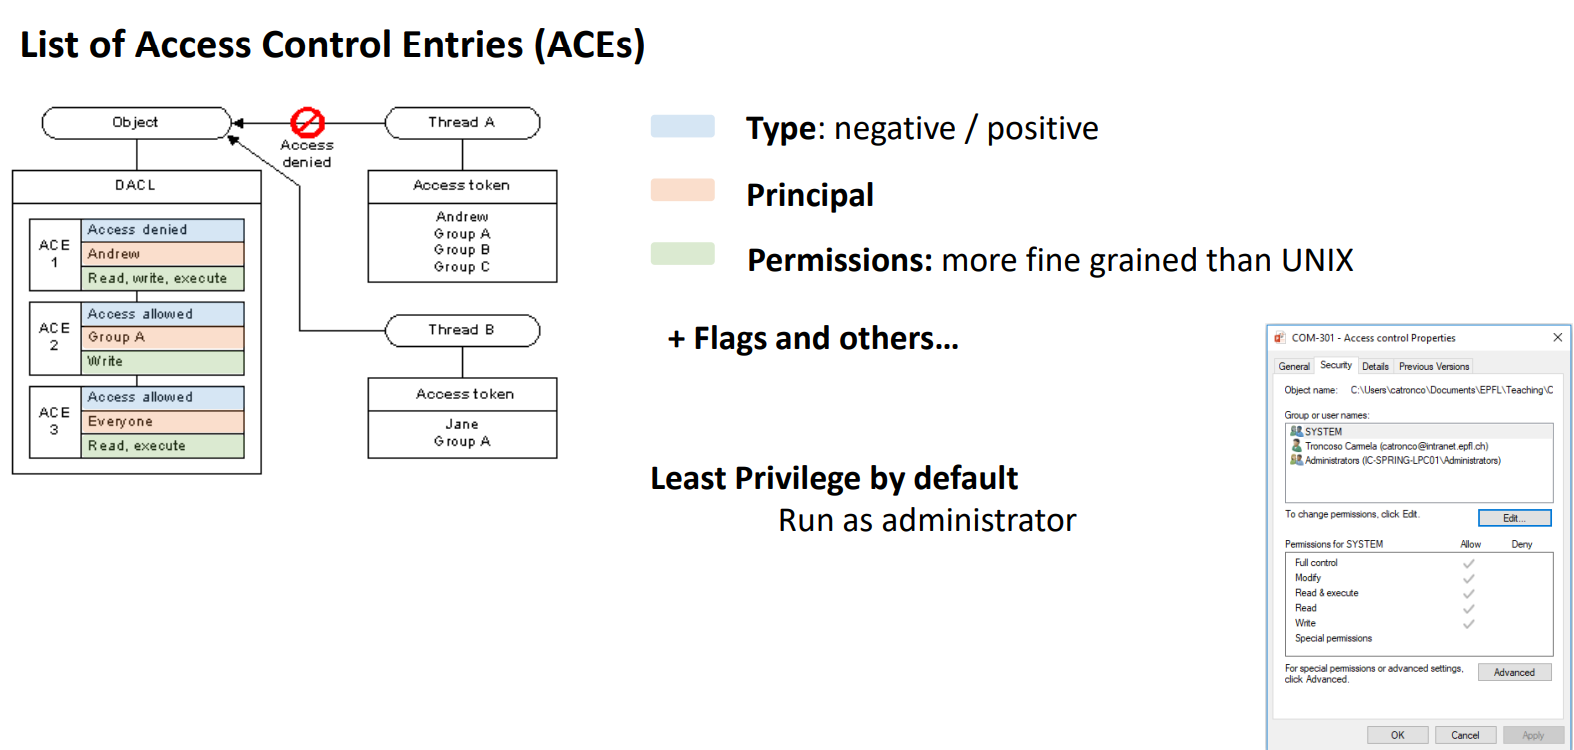
\includegraphics[width=\linewidth]{images/img_20261010_170445.png}
\end{center}

\begin{remark}[Why negative first?]
ACEs are evaluated \emph{in order}, and \textbf{negative ACEs are placed first}: an explicit denial must win over an allowance obtained through another entry (for instance, through a group). The same reasoning as for negative permissions in group-based access control applies.
\end{remark}

\paragraph{Least privilege by default.} Windows encourages least privilege through ``\emph{Run as administrator}'': even administrators work with a restricted token and elevate only when needed.

\subsection{Comparison UNIX vs.\ Windows}

\begin{table}[h]
\centering
\begin{tabular}{@{}p{3cm}p{5.2cm}p{5.2cm}@{}}
\toprule
 & \textbf{UNIX} & \textbf{Windows} \\
\midrule
\textbf{Per-object list} & 9 permission bits (owner/group/other) & DACL: list of ACEs (type, principal, permissions) \\[4pt]
\textbf{Granularity} & 3 actions (r, w, x) & More fine-grained permissions \\[4pt]
\textbf{Denials} & Implicit (first matching class decides) & Explicit negative ACEs, evaluated first \\[4pt]
\textbf{Subject side} & UID, GID(s) of the process & Access token (user, all groups recursively, privileges) \\[4pt]
\textbf{Elevation} & root, \texttt{sudo}/\texttt{su}, suid/sgid & ``Run as administrator'' \\
\bottomrule
\end{tabular}
\caption{DAC in UNIX and Windows.}
\end{table}

\section{Summary}

\begin{itemize}
    \item \textbf{Access control} ensures that all accesses of principals on objects are within the security policy; it is the \textbf{first line of defence} and is used at every layer (application, middleware, OS, hardware).
    \item It is split into \textbf{authentication} (bind the actor to a principal) and \textbf{authorization} (decide whether the principal may act); both are in the \textbf{TCB}.
    \item Do not write ``checks soup'': call a \textbf{reference monitor} (complete mediation, economy of mechanism).
    \item \textbf{DAC}: owners decide the permissions (Windows, Linux, macOS, social networks). \textbf{MAC}: a central policy decides.
    \item The \textbf{access control matrix} (subjects $\times$ objects $\to$ rights) is an abstract model, too big and sparse to implement directly.
    \item \textbf{ACLs}: permissions attached to objects (easy to see who accesses a resource, hard to audit a user). \textbf{Capabilities}: permissions attached to subjects (easy to audit and delegate, hard to revoke).
    \item \textbf{RBAC} (roles, one active role) and \textbf{groups} (union of all groups, negative permissions checked first) reduce the management cost of many subjects. RBAC suffers from role explosion, limited expressiveness and difficult separation of duty.
    \item \textbf{Ambient authority} is convenient but makes least privilege harder and causes the \textbf{confused deputy problem}. Solutions: re-check authorization in the privileged process, or use capabilities.
    \item \textbf{UNIX}: UIDs/GIDs, 9 permission bits (owner, group, other), check order owner $\to$ group $\to$ other, root never denied, directories have different semantics (list/add/traverse), \textbf{suid/sgid} (run with the owner's privileges; dangerous, in the TCB), \textbf{sticky bit} (restricted deletion, e.g., \texttt{/tmp}), \textbf{nobody} (safe user for untrusted code).
    \item \textbf{Windows}: DACL = list of ACEs (negative/positive, principal, fine-grained permissions), compared with the access token of the process; negative entries first.
\end{itemize}

